\documentclass[final,3p,times,twocolumn]{elsarticle}

%% Use the option review to obtain double line spacing
%% \documentclass[preprint,review,12pt]{elsarticle}

%% Use the options 1p,twocolumn; 3p; 3p,twocolumn; 5p; or 5p,twocolumn
%% for a journal layout:
%% \documentclass[final,1p,times]{elsarticle}
%% \documentclass[final,1p,times,twocolumn]{elsarticle}
%% \documentclass[final,3p,times]{elsarticle}
%% \documentclass[final,3p,times,twocolumn]{elsarticle}
%% \documentclass[final,5p,times]{elsarticle}
%% \documentclass[final,5p,times,twocolumn]{elsarticle}

%% if you use PostScript figures in your article
%% use the graphics package for simple commands
%% \usepackage{graphics}
%% or use the graphicx package for more complicated commands
%% \usepackage{graphicx}
%% or use the epsfig package if you prefer to use the old commands
%% \usepackage{epsfig}

%% The amssymb package provides various useful mathematical symbols
\usepackage{amssymb}
%% The amsthm package provides extended theorem environments
%% \usepackage{amsthm}
%% The bm package lets you access bold symbols in math mode using the \boldsymbol command (useful to get bold greek letters).
\usepackage{bm}
%% The bbm package is contains the indicator function symbol \mathbbm{1}
\usepackage{bbm}
%% The amsmath package contains the split environment, letting you split equations into multiple lines.
%% See "https://www.sharelatex.com/learn/Aligning_equations_with_amsmath " for an explanation.
\usepackage{amsmath}
%% The lineno packages adds line numbers. Start line numbering with
%% \begin{linenumbers}, end it with \end{linenumbers}. Or switch it on
%% for the whole article with \linenumbers after \end{frontmatter}.
%% \usepackage{lineno}
%% The algorithm defines the algorithm floating environment and the algpseudocode package is useful for constructing Pseudo code.
\usepackage{algorithm}
\usepackage{algpseudocode}
%% Declaring \argmin and \argmax operators:
\DeclareMathOperator*{\argmin}{arg\,min}
\DeclareMathOperator*{\argmax}{arg\,max}
%% natbib.sty is loaded by default. However, natbib options can be
%% provided with \biboptions{...} command. Following options are
%% valid:

%%   round  -  round parentheses are used (default)
%%   square -  square brackets are used   [option]
%%   curly  -  curly braces are used      {option}
%%   angle  -  angle brackets are used    <option>
%%   semicolon  -  multiple citations separated by semi-colon
%%   colon  - same as semicolon, an earlier confusion
%%   comma  -  separated by comma
%%   numbers-  selects numerical citations
%%   super  -  numerical citations as superscripts
%%   sort   -  sorts multiple citations according to order in ref. list
%%   sort&compress   -  like sort, but also compresses numerical citations
%%   compress - compresses without sorting
%%
%% \biboptions{comma,round}

% \biboptions{}


\journal{MPhil in Scientific Computing}

\begin{document}

\begin{frontmatter}

%% Title, authors and addresses

%% use the tnoteref command within \title for footnotes;
%% use the tnotetext command for the associated footnote;
%% use the fnref command within \author or \address for footnotes;
%% use the fntext command for the associated footnote;
%% use the corref command within \author for corresponding author footnotes;
%% use the cortext command for the associated footnote;
%% use the ead command for the email address,
%% and the form \ead[url] for the home page:
%%
%% \title{Title\tnoteref{label1}}
%% \tnotetext[label1]{}
%% \author{Name\corref{cor1}\fnref{label2}}
%% \ead{email address}
%% \ead[url]{home page}
%% \fntext[label2]{}
%% \cortext[cor1]{}
%% \address{Address\fnref{label3}}
%% \fntext[label3]{}

\title{Mini Project: Implementation and comparison of the Gaussian Mixture model, the K-means algorithm and the Dirichlet Process}

%% use optional labels to link authors explicitly to addresses:
%% \author[label1,label2]{<author name>}
%% \address[label1]{<address>}
%% \address[label2]{<address>}

\author{Brian Azizi}

\address{Cavendish Laboratory, Department of Physics, J J Thomson
  Avenue, Cambridge. CB3 0HE}

\begin{abstract}
Abstract of the mini project. As part of the written assignment for the MPhil in Scientific Computing, I have implemented three clustering algorithms in the C++ programming language, the k-means algorithm, the Gaussian mixture model and the Dirichlet Process mixture model. Subsequently, the algorithms will be compared and texted on a number of data sets.
\end{abstract}

\end{frontmatter}

%%
%% Start line numbering here if you want
%%
% \linenumbers

%% main text
\section{Introduction}
\label{sect:Intro}
The goal of \emph{clustering} is to discover structure in the data by identifying groups of similar data points. 
Clustering has found applications in biology (gene clustering), market research (market segmentation), grouping similar news (news clustering, eg Google News) and image segmentation (which has applications in medicine).

We begin by introducing a very simple clustering algorithm: K-Means. 
Then we make a small digression to discuss the related problem of density estimation (and outlier detection) which will lead to the Mixture of Gaussians model.
Finally, we take a Bayesian non-parametric approach and discuss the Dirichlet Process Mixture Model.

Throughout this report, we assume we have a dataset $\{\boldsymbol x^{(i)}\}_{i=1}^N$ consisting of $N$ observations of a random variable $\boldsymbol x$ living in $D$-dimensional Euclidean space, $\mathbb{R}^D$.
 




\section{K-Means Clustering}
\emph{K-Means} is the simplest clustering algorithm.
We assume there exists $K$ clusters, and we introduce $K$ \emph{cluster centroids} $\boldsymbol \mu_k \in \mathbb{R}^D$.
These centroids can be thought of as representatives of the individual clusters (or as their centres, as we will soon see).
We denote the label, or \emph{cluster assignment}, of the $i$th training sample by $c^{(i)} \in \{1, \dots, K\}$. 

\subsection{The K-Means algorithm}

The K-Means algorithm begins with an initial guess for the $\boldsymbol \mu_k$. 
We then repeat the following two steps until convergence.
First, we assign each data point to the nearest cluster centroid.
Second, we update each cluster centroid to be the mean of all the points assigned to them.
Algorithm \ref{alg:kmeans} contains the pseudo-code.

\begin{algorithm}
\caption{K-Means algorithm}
\label{alg:kmeans}
\begin{algorithmic}[1]
\Procedure{K-Means}{$X,K$}
\State{Randomly initialize $K$ cluster centroids in $\mathbb{R}^D$}
\Repeat
\For{$i = 1:N$}\Comment
\State{$c^{(i)} = \argmin_k ||\boldsymbol{x}_i - \boldsymbol{k}_k||$}
\EndFor
\For{$k = 1:K$}
\State{$N_k = \sum_{i=1}^N \mathbbm{1}\{c^{(i)} = k \}$}
\State{$\boldsymbol{\mu}_k = \sum_{i:c^{(i)}=k} \boldsymbol{x}^{(i)} / N_k$}
\EndFor
\Until{Convergence}\Comment{No more changes}
\EndProcedure \\
\Return{$c^{(1)}, \dots, c^{(N)}, \boldsymbol{\mu}_1, \dots, \boldsymbol{\mu}_K $}
\end{algorithmic}
\end{algorithm}

\subsection{Convergence of K-Means}

In order to show convergence, we can cast the K-Means problem into an optimization problem. Define the \emph{distortion function} 
\begin{equation}
J(\boldsymbol c, \boldsymbol \mu) = \sum_{i=1}^N ||\boldsymbol x^{(i)} - \boldsymbol \mu_{c^{(i)}}||^2
\label{eqn:distortion}
\end{equation}
The K-Means problem is then equivalent to minimizing the distortion function and the K-Means algorithm corresponds to performing coordinate descent on $J(\boldsymbol c, \boldsymbol \mu)$.
Thus, the algorithm is guaranteed to converge. 
Figure \ref{fig:kmeans1} shows a result from running K-Means to convergence with $K = 3$.
\begin{figure}
\centering
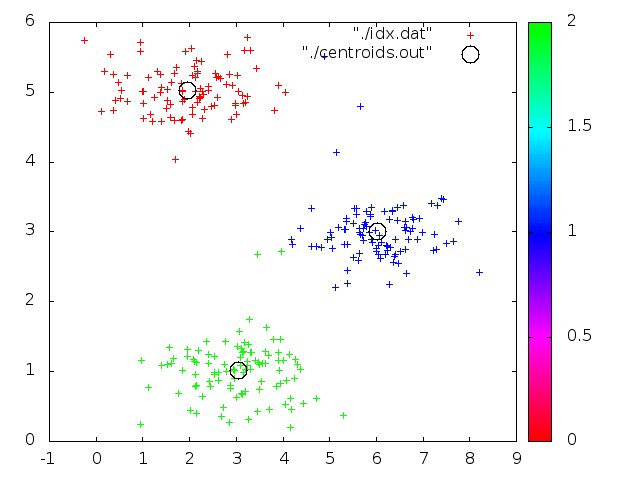
\includegraphics[width=3in]{kmeans1.png}
\caption{Result of running the K-Means algorithm on the toyclusters dataset with $K=3$}
\label{fig:kmeans1}
\end{figure}

However, it is possible for the K-Means algorithm to get stuck in local optima.
Figure \ref{fig:kmeans2} is the same as figure \ref{fig:kmeans1} but with a different initialization for the cluster centroids. 
\begin{figure}
\centering
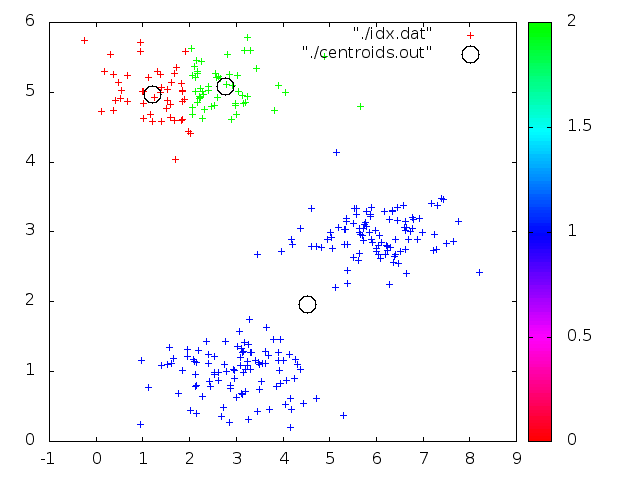
\includegraphics[width=3in]{kmeans2.png}
\caption{Local optimum of K-Means algorithm ($K=3$).}
\label{fig:kmeans2}
\end{figure}
In practice, we deal with this problem by performing several run of the entire K-Means algorithm, each with different initializations of the cluster centroids, and then choosing the output for which the distortion measure is smallest.

Note on K-Medoids.

\subsection{Model selection for K-Means}
The K-means model has only one hyperparameter, namely the number of clusters $K$.
In practice, $K$ is often chosen manually.
In some applications, we have prior knowledge about the number of clusters.
There exist some model selection tools, most notably the elbow method.
If, during the algorithm, a cluster ends up being empty, we can either remove it or just randomly reinitialize the centroid.

For more information on K-Means clustering, see \cite{Bishop}.


\section{The Gaussian Mixture Model}
The Gaussian mixture model (GMM) (also known as mixtures of Gaussians) is the most widely used mixture model.
Before we explore its applications to clustering, let us first discuss the related problem of density estimation.
The goal of density estimation is to build the density $p(\boldsymbol x)$ of the random variable $\boldsymbol x \in \mathbb{R}^D$, given a set $\{\boldsymbol x^{(i)}\}_{i=1}^N$ of $N$ observations of $\boldsymbol x$.

Once we have formed the density $p(\boldsymbol x)$, we can apply the model to the problem of \emph{anomaly detection}.
Given a new observation $\boldsymbol x^{(N+1)}$, we flag it as an anomaly if $p(\boldsymbol x^{(N+1)}) < \epsilon$, where $\epsilon > 0$ is a pre-defined threshold.

The classical approach to density estimation is to assume $p(\boldsymbol x)$ belongs to some parametric family of distributions and to then infer the parameters from the data using tools such as \emph{maximum likelihood estimation}. 

\subsection{Modelling densities as mixtures of Gaussians}

What do we do if our data does not seem to come from any of the standard distributions (eg figure \ref{fig:gmm1}).
\begin{figure}
\centering
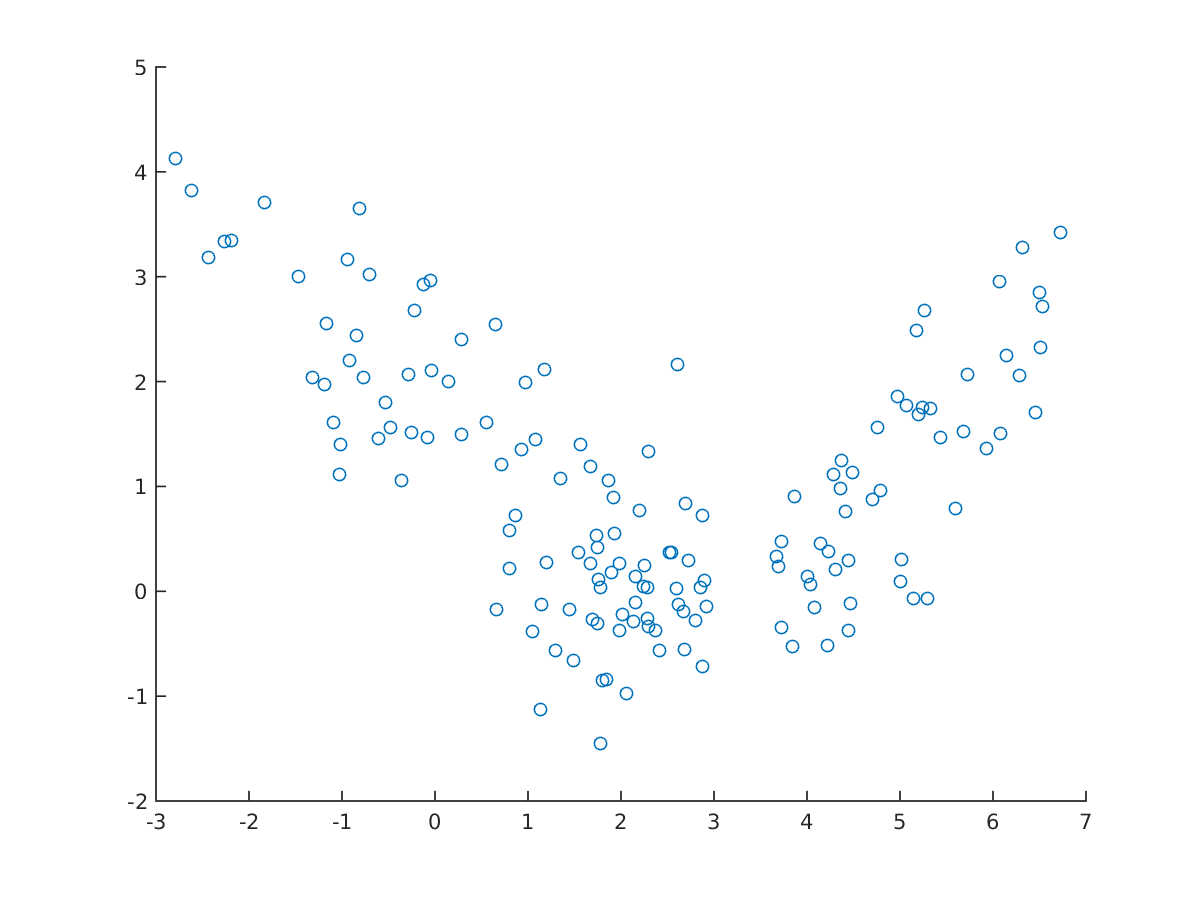
\includegraphics[width=3in]{gmm1.png}
%\caption{}
\label{fig:gmm1}
\end{figure}
One approach is to do non-parametric density estimation. A more straight forward strategy is to use a mixture model.
In the GMM, we assume that the data was generated from $K$ distinct Gaussian \emph{base distributions}. 
We do not know which Gaussian generated which data points, so we introduce the discrete latent variable $z^{(i)} \in \{1,2,\dots,K\}$ that tells us which cluster sample $\boldsymbol x^{(i)}$ belongs to.

We assume that 
\begin{equation}
z \sim Discrete(\,\boldsymbol \pi)
\label{eqnzdistro}
\end{equation}
\begin{equation}
\boldsymbol x \,|\, z \sim \mathcal{N}(\,\boldsymbol{\mu_z}, \boldsymbol \Sigma_z)
\label{eqn:x|z-distro}
\end{equation}
This means
\begin{equation}
p(z) = \pi_z, \qquad \pi_k > 0 \, \forall k \in \{1,\dots,K\}, \sum_{k=1}^K \pi_k = 1 
\end{equation}
\begin{equation}
\begin{split}
p(\boldsymbol x\,|\,z) &= \mathcal{N}(\boldsymbol x\,|\, \boldsymbol \mu_z, \boldsymbol \Sigma_z) \\
&= \frac{1}{\sqrt{2\pi\,|\Sigma_z|}}\exp(-\frac{1}{2}(\boldsymbol x - \boldsymbol \mu_z)^T\boldsymbol \Sigma_z^{-1} (\boldsymbol x - \boldsymbol \mu_z))\\
\end{split}
\end{equation}

From the sum rule and product rule of probability, we have
\begin{equation}
\begin{split}
p(\boldsymbol x) &= \sum_z p(\boldsymbol x, z) \\
&= \sum_z p(z)p(\boldsymbol x \,|\, z)\\
&= \sum_{k=1}^K \pi_k \mathcal{N}(\boldsymbol x\,|\,\boldsymbol \mu_k, \boldsymbol \Sigma_k)
\label{eqn:gmmdensity}
\end{split}
\end{equation}

\subsection{The EM algorithm for the GMM}
Given a training set $S$, how to we fit the model parameters $\{\pi_k, \boldsymbol \mu_k, \boldsymbol \Sigma_k; k=1,\dots,K\}$?
	If the labels $z^{(i)}$ were observed, we could formulate the likelihood of the data \footnote{In this case the model is equivalent to the quadratic discriminant analysis model used for classification} 
\begin{equation}
\mathcal{L}(\pi_k, \boldsymbol \mu_k, \boldsymbol \Sigma_k) = \prod_{i=1}^N p(\boldsymbol x^{(i)},z^{(i)}\,|\,\pi_k, \boldsymbol \mu_k, \boldsymbol \Sigma_k)
\label{eqn:LDAlikelihood}
\end{equation}
Maximising the likelihood would yield the following solutions for $k = 1,\dots,K$:
\begin{equation}
\begin{split}
&\pi_k = \frac{\sum_{i=1}^N \mathbbm{1}\{z^{(i)} = k\}}{N}\\
&\mu_k = \frac{\sum_{i=1}^N \mathbbm{1}\{z^{(i)} = k\} \boldsymbol{x}^{(i)}}{\sum_{i=1}^N \mathbbm{1}\{z^{(i)} = k\}}\\
&\Sigma_k = \frac{\sum_{i=1}^N \mathbbm{1}\{z^{(i)} = k\} (\boldsymbol{x}^{(i)} - \boldsymbol \mu_k)(\boldsymbol{x}^{(i)} - \boldsymbol \mu_k)^T}{\sum_{i=1}^N \mathbbm{1}\{z^{(i)} = k\}}\\
\end{split}
\end{equation}
(See the appendix for a derivation.)

In the unsupervised setting, we do not observe the values of $z^{(i)}$. 
Thus, the likelihood of our data now takes the form
\begin{equation}
	\mathcal{L}(\boldsymbol \pi, \boldsymbol \mu, \boldsymbol \Sigma) = \prod_{i=1}^N p(\boldsymbol x^{(i)}\,|\,\boldsymbol \pi, \boldsymbol \mu, \boldsymbol \Sigma)\\
\label{eqn:gmmLikelihood}
\end{equation}
Taking logs on both side and using equation \ref{eqn:gmmdensity}, we can formulate our objective function as
\begin{equation}
\begin{split}
\log\mathcal{L}(\boldsymbol \pi, \boldsymbol \mu, \boldsymbol \Sigma) &= \sum_{i=1}^N \log p(\boldsymbol x^{(i)}\,|\,\boldsymbol \pi \boldsymbol \mu, \boldsymbol \Sigma)\\
&= \sum_{i=1}^N \log \left(\sum_{k=1}^K \pi_k \mathcal{N}(\boldsymbol x^{(i)}\,|\, \boldsymbol \mu_k, \boldsymbol \Sigma_k)\right)\\
\end{split}
\label{eqn:gmmlogLikelihood}
\end{equation}

Maximising this objective function directly is problematic due to summation inside the logarithm term and there is, in fact, no known closed form solution.
Instead we us an iterative scheme in which we first formulate a ``guess" for the $z^{(i)}$ given our current parameter values and then find the optimal model parameters given our guess. 



\section*{Acknowledgements}
Here I acknowledge the assistance of my supervisor, my industrial sponsor,
and the effects of caffine on my ability to produce this report on time.

%% The Appendices part is started with the command \appendix;
%% appendix sections are then done as normal sections
\appendix

\section{On the Derivation of the Quadratic Formula}
\label{app:quad}

%% References
%%
%% Following citation commands can be used in the body text:
%% Usage of \cite is as follows:
%%   \cite{key}         ==>>  [#]
%%   \cite[chap. 2]{key} ==>> [#, chap. 2]
%%

%% References with bibTeX database:
\section*{Bibliography}
\bibliographystyle{elsarticle-num}
\bibliography{references.bib}

%% Authors are advised to submit their bibtex database files. They are
%% requested to list a bibtex style file in the manuscript if they do
%% not want to use elsarticle-num.bst.

%% References without bibTeX database:

% \begin{thebibliography}{00}

%% \bibitem must have the following form:
%%   \bibitem{key}...
%%

% \bibitem{}

% \end{thebibliography}


\end{document}

%%
%% End of file `mini.tex'.